\chapter{Presentation}

% Chapter-wide image
\begin{center}
    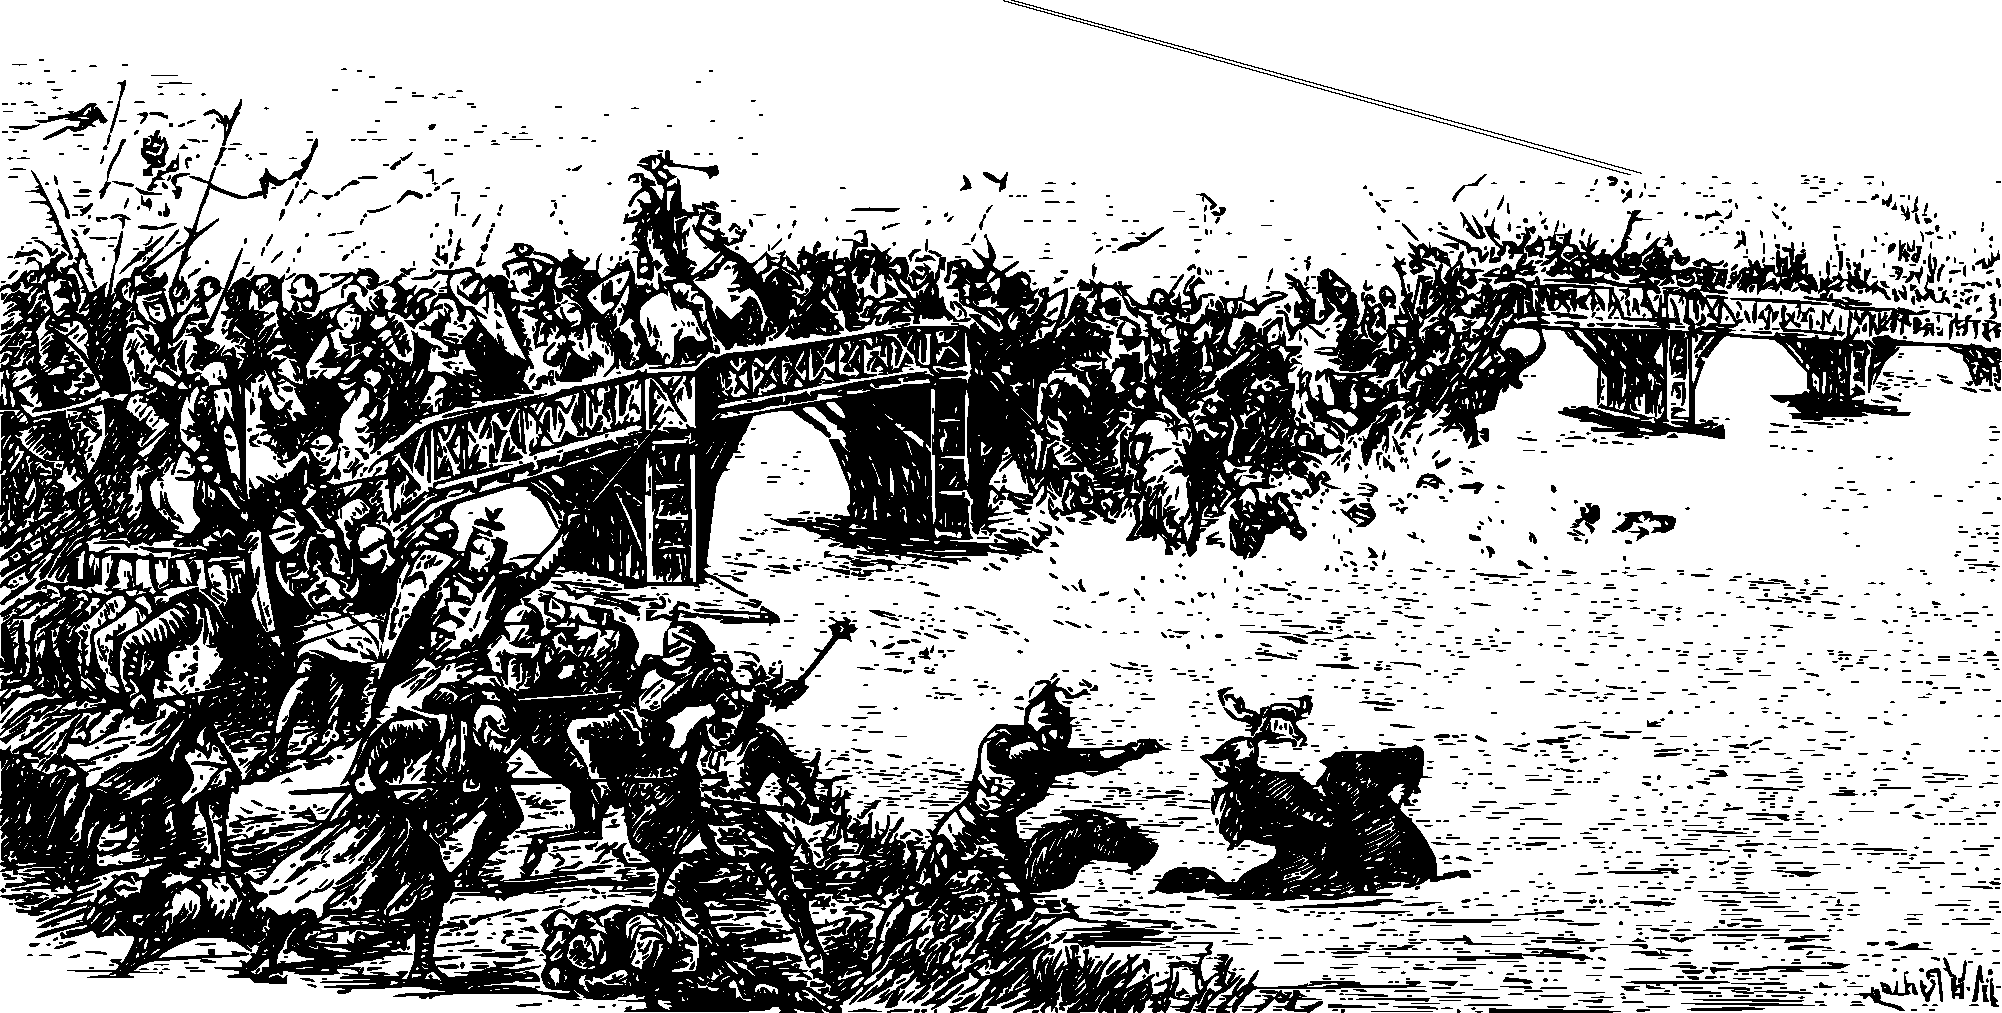
\includegraphics[width=\textwidth]{./images/presentation01.pdf}
\end{center}

% \marginnote{\small \textit{Note: These margins are designed to allow space for important notations and additional context.}}

In the realm of tabletop role-playing games, Eidos stands as a unique and innovative addition to the genre. Rooted in open-source principles, this game is designed to be both immersive and accessible...

The character creation process in Eidos is a deep and engaging experience, allowing players to build their characters from the ground up. With character sheets devoted to personality, religion, physical description, background, clothing, equipment, and skills, players have the tools to create a truly unique and memorable character.

The combat system in Eidos is designed to be immersive and engaging, with mechanics that are designed to create dynamic and exciting combat scenes. The game's mechanics are based on classic combat narratives, and the system strives to be a simulation of combat rather than simply a turn-based dice-rolling game. The standard rules are designed to be played in a pre-modern low-fantasy setting, but the game is easily adaptable to other role-playing scenarios.

This rulebook is divided into ten chapters, each covering a crucial aspect of the game. Chapters 1 through 6 establish the core elements of character creation: Chapter 1: Personality deals with alignments, beliefs, and personal traits; Chapter 2: Spirituality and Religion outlines faith adherence, tolerance, demeanor, and organizational roles; Chapter 3: Physical Description covers a character's aesthetics; Chapter 4: Skills outlines specialized training and advancement; Chapter 5: Background details prompts for backstory and narrative origins; and Chapter 6: Clothing and Equipment details active armor mechanics, shields, weapons, and standard adventuring gear tables.

\begin{figure}[h]
    \centering
    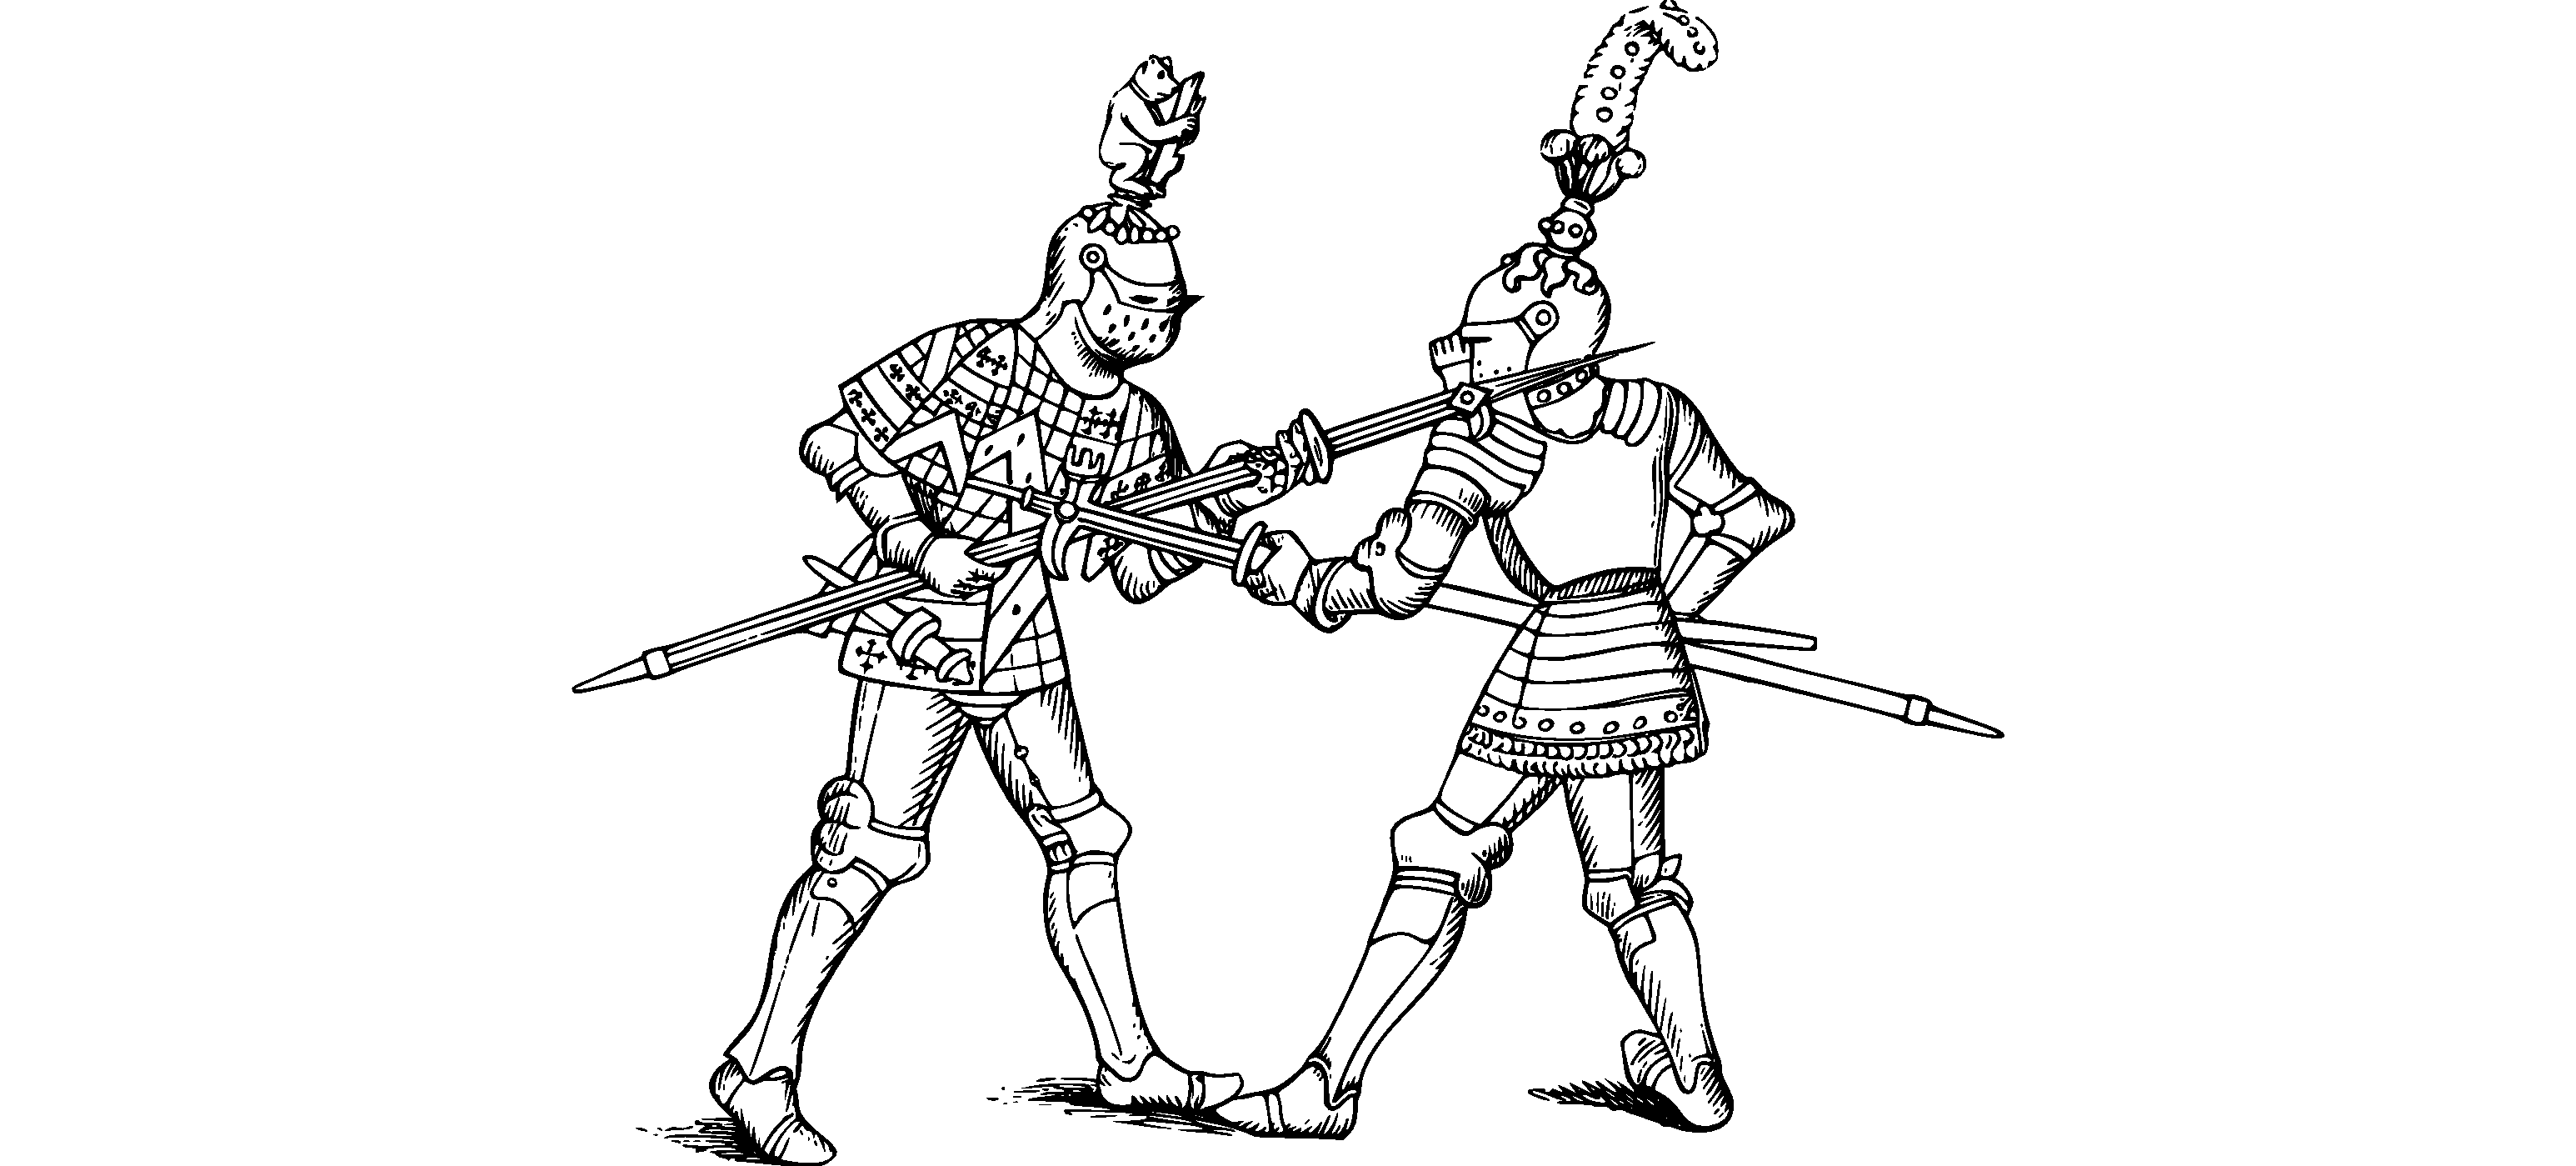
\includegraphics[width=\textwidth]{./images/presentation02.pdf}
    % \caption{Inline Example Image}
\end{figure}

The remaining chapters detail the core systems of play and administration: Chapter 7: Conflict Mechanics governs the 2d20 core resolution roll, combat actions, active defenses, and detailed critical injury tables; Chapter 8: Survival Mechanics details fatigue, overland travel, scavenging, and recovery from trauma; Chapter 9: Game Master Tools provides advice and quick templates for world-building, NPCs, and encounter scaling; and Chapter 10: Magic and Optional Rules details spellcasting, spell lists, mana mechanics, and tactical combat alternatives.

In conclusion, Eidos is an open source tabletop RPG system that offers a unique and engaging narrative experience, with mechanics that are designed to create immersive and exciting combat scenes. With its deep character creation process, engaging combat mechanics, and comprehensive survival mechanics, Eidos is a game that offers endless possibilities for players to explore and experience.

